\documentclass[1p]{elsarticle_modified}
%\bibliographystyle{elsarticle-num}

%\usepackage[colorlinks]{hyperref}
%\usepackage{abbrmath_seonhwa} %\Abb, \Ascr, \Acal ,\Abf, \Afrak
\usepackage{amsfonts}
\usepackage{amssymb}
\usepackage{amsmath}
\usepackage{amsthm}
\usepackage{scalefnt}
\usepackage{amsbsy}
\usepackage{kotex}
\usepackage{caption}
\usepackage{subfig}
\usepackage{color}
\usepackage{graphicx}
\usepackage{xcolor} %% white, black, red, green, blue, cyan, magenta, yellow
\usepackage{float}
\usepackage{setspace}
\usepackage{hyperref}

\usepackage{tikz}
\usetikzlibrary{arrows}

\usepackage{multirow}
\usepackage{array} % fixed length table
\usepackage{hhline}

%%%%%%%%%%%%%%%%%%%%%
\makeatletter
\renewcommand*\env@matrix[1][\arraystretch]{%
	\edef\arraystretch{#1}%
	\hskip -\arraycolsep
	\let\@ifnextchar\new@ifnextchar
	\array{*\c@MaxMatrixCols c}}
\makeatother %https://tex.stackexchange.com/questions/14071/how-can-i-increase-the-line-spacing-in-a-matrix
%%%%%%%%%%%%%%%

\usepackage[normalem]{ulem}

\newcommand{\msout}[1]{\ifmmode\text{\sout{\ensuremath{#1}}}\else\sout{#1}\fi}
%SOURCE: \msout is \stkout macro in https://tex.stackexchange.com/questions/20609/strikeout-in-math-mode

\newcommand{\cancel}[1]{
	\ifmmode
	{\color{red}\msout{#1}}
	\else
	{\color{red}\sout{#1}}
	\fi
}

\newcommand{\add}[1]{
	{\color{blue}\uwave{#1}}
}

\newcommand{\replace}[2]{
	\ifmmode
	{\color{red}\msout{#1}}{\color{blue}\uwave{#2}}
	\else
	{\color{red}\sout{#1}}{\color{blue}\uwave{#2}}
	\fi
}

\newcommand{\Sol}{\mathcal{S}} %segment
\newcommand{\D}{D} %diagram
\newcommand{\A}{\mathcal{A}} %arc


%%%%%%%%%%%%%%%%%%%%%%%%%%%%%5 test

\def\sl{\operatorname{\textup{SL}}(2,\Cbb)}
\def\psl{\operatorname{\textup{PSL}}(2,\Cbb)}
\def\quan{\mkern 1mu \triangleright \mkern 1mu}

\theoremstyle{definition}
\newtheorem{thm}{Theorem}[section]
\newtheorem{prop}[thm]{Proposition}
\newtheorem{lem}[thm]{Lemma}
\newtheorem{ques}[thm]{Question}
\newtheorem{cor}[thm]{Corollary}
\newtheorem{defn}[thm]{Definition}
\newtheorem{exam}[thm]{Example}
\newtheorem{rmk}[thm]{Remark}
\newtheorem{alg}[thm]{Algorithm}

\newcommand{\I}{\sqrt{-1}}
\begin{document}

%\begin{frontmatter}
%
%\title{Boundary parabolic representations of knots up to 8 crossings}
%
%%% Group authors per affiliation:
%\author{Yunhi Cho} 
%\address{Department of Mathematics, University of Seoul, Seoul, Korea}
%\ead{yhcho@uos.ac.kr}
%
%
%\author{Seonhwa Kim} %\fnref{s_kim}}
%\address{Center for Geometry and Physics, Institute for Basic Science, Pohang, 37673, Korea}
%\ead{ryeona17@ibs.re.kr}
%
%\author{Hyuk Kim}
%\address{Department of Mathematical Sciences, Seoul National University, Seoul 08826, Korea}
%\ead{hyukkim@snu.ac.kr}
%
%\author{Seokbeom Yoon}
%\address{Department of Mathematical Sciences, Seoul National University, Seoul, 08826,  Korea}
%\ead{sbyoon15@snu.ac.kr}
%
%\begin{abstract}
%We find all boundary parabolic representation of knots up to 8 crossings.
%
%\end{abstract}
%\begin{keyword}
%    \MSC[2010] 57M25 
%\end{keyword}
%
%\end{frontmatter}

%\linenumbers
%\tableofcontents
%
\newcommand\colored[1]{\textcolor{white}{\rule[-0.35ex]{0.8em}{1.4ex}}\kern-0.8em\color{red} #1}%
%\newcommand\colored[1]{\textcolor{white}{ #1}\kern-2.17ex	\textcolor{white}{ #1}\kern-1.81ex	\textcolor{white}{ #1}\kern-2.15ex\color{red}#1	}

{\Large $\underline{12a_{0555}~(K12a_{0555})}$}

\setlength{\tabcolsep}{10pt}
\renewcommand{\arraystretch}{1.6}
\vspace{1cm}\begin{tabular}{m{100pt}>{\centering\arraybackslash}m{274pt}}
\multirow{5}{120pt}{
	\centering
	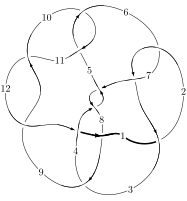
\includegraphics[width=112pt]{../../../GIT/diagram.site/Diagrams/png/1356_12a_0555.png}\\
\ \ \ A knot diagram\footnotemark}&
\allowdisplaybreaks
\textbf{Linearized knot diagam} \\
\cline{2-2}
 &
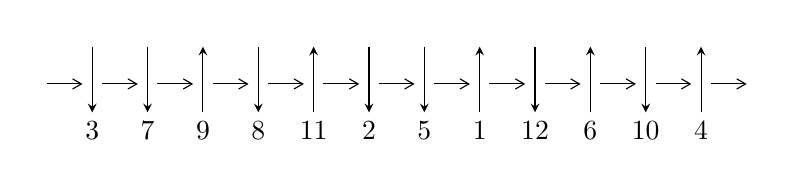
\begin{tikzpicture}[x=20pt, y=17pt]
	% nodes
	\node (C0) at (0, 0) {};
	\node (C1) at (1, 0) {};
	\node (C1U) at (1, +1) {};
	\node (C1D) at (1, -1) {3};

	\node (C2) at (2, 0) {};
	\node (C2U) at (2, +1) {};
	\node (C2D) at (2, -1) {7};

	\node (C3) at (3, 0) {};
	\node (C3U) at (3, +1) {};
	\node (C3D) at (3, -1) {9};

	\node (C4) at (4, 0) {};
	\node (C4U) at (4, +1) {};
	\node (C4D) at (4, -1) {8};

	\node (C5) at (5, 0) {};
	\node (C5U) at (5, +1) {};
	\node (C5D) at (5, -1) {11};

	\node (C6) at (6, 0) {};
	\node (C6U) at (6, +1) {};
	\node (C6D) at (6, -1) {2};

	\node (C7) at (7, 0) {};
	\node (C7U) at (7, +1) {};
	\node (C7D) at (7, -1) {5};

	\node (C8) at (8, 0) {};
	\node (C8U) at (8, +1) {};
	\node (C8D) at (8, -1) {1};

	\node (C9) at (9, 0) {};
	\node (C9U) at (9, +1) {};
	\node (C9D) at (9, -1) {12};

	\node (C10) at (10, 0) {};
	\node (C10U) at (10, +1) {};
	\node (C10D) at (10, -1) {6};

	\node (C11) at (11, 0) {};
	\node (C11U) at (11, +1) {};
	\node (C11D) at (11, -1) {10};

	\node (C12) at (12, 0) {};
	\node (C12U) at (12, +1) {};
	\node (C12D) at (12, -1) {4};
	\node (C13) at (13, 0) {};

	% arrows
	\draw[->,>={angle 60}]
	(C0) edge (C1) (C1) edge (C2) (C2) edge (C3) (C3) edge (C4) (C4) edge (C5) (C5) edge (C6) (C6) edge (C7) (C7) edge (C8) (C8) edge (C9) (C9) edge (C10) (C10) edge (C11) (C11) edge (C12) (C12) edge (C13) ;	\draw[->,>=stealth]
	(C1U) edge (C1D) (C2U) edge (C2D) (C3D) edge (C3U) (C4U) edge (C4D) (C5D) edge (C5U) (C6U) edge (C6D) (C7U) edge (C7D) (C8D) edge (C8U) (C9U) edge (C9D) (C10D) edge (C10U) (C11U) edge (C11D) (C12D) edge (C12U) ;
	\end{tikzpicture} \\
\hhline{~~} \\& 
\textbf{Solving Sequence} \\ \cline{2-2} 
 &
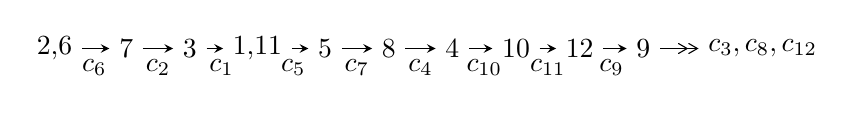
\begin{tikzpicture}[x=23pt, y=7pt]
	% node
	\node (A0) at (-1/8, 0) {2,6};
	\node (A1) at (1, 0) {7};
	\node (A2) at (2, 0) {3};
	\node (A3) at (49/16, 0) {1,11};
	\node (A4) at (33/8, 0) {5};
	\node (A5) at (41/8, 0) {8};
	\node (A6) at (49/8, 0) {4};
	\node (A7) at (57/8, 0) {10};
	\node (A8) at (65/8, 0) {12};
	\node (A9) at (73/8, 0) {9};
	\node (C1) at (1/2, -1) {$c_{6}$};
	\node (C2) at (3/2, -1) {$c_{2}$};
	\node (C3) at (5/2, -1) {$c_{1}$};
	\node (C4) at (29/8, -1) {$c_{5}$};
	\node (C5) at (37/8, -1) {$c_{7}$};
	\node (C6) at (45/8, -1) {$c_{4}$};
	\node (C7) at (53/8, -1) {$c_{10}$};
	\node (C8) at (61/8, -1) {$c_{11}$};
	\node (C9) at (69/8, -1) {$c_{9}$};
	\node (A10) at (11, 0) {$c_{3},c_{8},c_{12}$};

	% edge
	\draw[->,>=stealth]	
	(A0) edge (A1) (A1) edge (A2) (A2) edge (A3) (A3) edge (A4) (A4) edge (A5) (A5) edge (A6) (A6) edge (A7) (A7) edge (A8) (A8) edge (A9) ;
	\draw[->>,>={angle 60}]	
	(A9) edge (A10);
\end{tikzpicture} \\ 

\end{tabular} \\

\footnotetext{
The image of knot diagram is generated by the software ``\textbf{Draw programme}" developed by Andrew Bartholomew(\url{http://www.layer8.co.uk/maths/draw/index.htm\#Running-draw}), where we modified some parts for our purpose(\url{https://github.com/CATsTAILs/LinksPainter}).
}\phantom \\ \newline 
\centering \textbf{Ideals for irreducible components\footnotemark of $X_{\text{par}}$} 
 
\begin{align*}
I^u_{1}&=\langle 
1.57592\times10^{318} u^{123}-2.08157\times10^{318} u^{122}+\cdots+2.25880\times10^{319} b-3.26705\times10^{319},\\
\phantom{I^u_{1}}&\phantom{= \langle  }3.30221\times10^{318} u^{123}-4.03875\times10^{318} u^{122}+\cdots+2.25880\times10^{319} a-1.14717\times10^{320},\;u^{124}- u^{123}+\cdots-13 u+1\rangle \\
I^u_{2}&=\langle 
7 u^{27}-42 u^{25}+\cdots+16 u^3+b,\;24 u^{27}-13 u^{26}+\cdots+a+27,\;u^{28}-7 u^{26}+\cdots+u+1\rangle \\
\\
\end{align*}
\raggedright * 2 irreducible components of $\dim_{\mathbb{C}}=0$, with total 152 representations.\\
\footnotetext{All coefficients of polynomials are rational numbers. But the coefficients are sometimes approximated in decimal forms when there is not enough margin.}
\newpage
\renewcommand{\arraystretch}{1}
\centering \section*{I. $I^u_{1}= \langle 1.58\times10^{318} u^{123}-2.08\times10^{318} u^{122}+\cdots+2.26\times10^{319} b-3.27\times10^{319},\;3.30\times10^{318} u^{123}-4.04\times10^{318} u^{122}+\cdots+2.26\times10^{319} a-1.15\times10^{320},\;u^{124}- u^{123}+\cdots-13 u+1 \rangle$}
\flushleft \textbf{(i) Arc colorings}\\
\begin{tabular}{m{7pt} m{180pt} m{7pt} m{180pt} }
\flushright $a_{2}=$&$\begin{pmatrix}0\\u\end{pmatrix}$ \\
\flushright $a_{6}=$&$\begin{pmatrix}1\\0\end{pmatrix}$ \\
\flushright $a_{7}=$&$\begin{pmatrix}1\\u^2\end{pmatrix}$ \\
\flushright $a_{3}=$&$\begin{pmatrix}- u\\- u^3+u\end{pmatrix}$ \\
\flushright $a_{1}=$&$\begin{pmatrix}u^3\\u^5- u^3+u\end{pmatrix}$ \\
\flushright $a_{11}=$&$\begin{pmatrix}-0.146193 u^{123}+0.178800 u^{122}+\cdots-13.8891 u+5.07865\\-0.0697681 u^{123}+0.0921538 u^{122}+\cdots-10.2467 u+1.44636\end{pmatrix}$ \\
\flushright $a_{5}=$&$\begin{pmatrix}-0.356991 u^{123}+0.445191 u^{122}+\cdots-55.4783 u+6.75271\\-0.119813 u^{123}+0.134953 u^{122}+\cdots-19.0220 u+1.00634\end{pmatrix}$ \\
\flushright $a_{8}=$&$\begin{pmatrix}-0.547390 u^{123}+0.484893 u^{122}+\cdots-80.7903 u-2.39707\\-0.0369578 u^{123}+0.0165463 u^{122}+\cdots-1.32633 u-2.40645\end{pmatrix}$ \\
\flushright $a_{4}=$&$\begin{pmatrix}0.547878 u^{123}-0.540683 u^{122}+\cdots+90.4297 u-9.53174\\0.286119 u^{123}-0.265471 u^{122}+\cdots+37.8431 u-1.66144\end{pmatrix}$ \\
\flushright $a_{10}=$&$\begin{pmatrix}-0.0764246 u^{123}+0.0866464 u^{122}+\cdots-3.64233 u+3.63229\\-0.0697681 u^{123}+0.0921538 u^{122}+\cdots-10.2467 u+1.44636\end{pmatrix}$ \\
\flushright $a_{12}=$&$\begin{pmatrix}-0.473969 u^{123}+0.562191 u^{122}+\cdots-75.5693 u+7.83665\\-0.174923 u^{123}+0.183416 u^{122}+\cdots-28.4694 u+1.00218\end{pmatrix}$ \\
\flushright $a_{9}=$&$\begin{pmatrix}-0.547891 u^{123}+0.484216 u^{122}+\cdots-80.7327 u-2.40114\\-0.0395895 u^{123}+0.0231613 u^{122}+\cdots-1.15575 u-2.46193\end{pmatrix}$\\&\end{tabular}
\flushleft \textbf{(ii) Obstruction class $= -1$}\\~\\
\flushleft \textbf{(iii) Cusp Shapes $= -0.236486 u^{123}+0.153343 u^{122}+\cdots+23.5886 u-7.90116$}\\~\\
\newpage\renewcommand{\arraystretch}{1}
\flushleft \textbf{(iv) u-Polynomials at the component}\newline \\
\begin{tabular}{m{50pt}|m{274pt}}
Crossings & \hspace{64pt}u-Polynomials at each crossing \\
\hline $$\begin{aligned}c_{1}\end{aligned}$$&$\begin{aligned}
&u^{124}+45 u^{123}+\cdots-65 u+1
\end{aligned}$\\
\hline $$\begin{aligned}c_{2},c_{6}\end{aligned}$$&$\begin{aligned}
&u^{124}- u^{123}+\cdots-13 u+1
\end{aligned}$\\
\hline $$\begin{aligned}c_{3}\end{aligned}$$&$\begin{aligned}
&u^{124}-18 u^{122}+\cdots+83060 u+9129
\end{aligned}$\\
\hline $$\begin{aligned}c_{4},c_{7}\end{aligned}$$&$\begin{aligned}
&u^{124}-2 u^{123}+\cdots-570346 u+135173
\end{aligned}$\\
\hline $$\begin{aligned}c_{5},c_{10}\end{aligned}$$&$\begin{aligned}
&u^{124}+u^{123}+\cdots+u+1
\end{aligned}$\\
\hline $$\begin{aligned}c_{8}\end{aligned}$$&$\begin{aligned}
&u^{124}+11 u^{123}+\cdots+19900 u+5329
\end{aligned}$\\
\hline $$\begin{aligned}c_{9},c_{11}\end{aligned}$$&$\begin{aligned}
&u^{124}+37 u^{123}+\cdots+31 u+1
\end{aligned}$\\
\hline $$\begin{aligned}c_{12}\end{aligned}$$&$\begin{aligned}
&u^{124}+9 u^{123}+\cdots+54702 u+6689
\end{aligned}$\\
\hline
\end{tabular}\\~\\
\newpage\renewcommand{\arraystretch}{1}
\flushleft \textbf{(v) Riley Polynomials at the component}\newline \\
\begin{tabular}{m{50pt}|m{274pt}}
Crossings & \hspace{64pt}Riley Polynomials at each crossing \\
\hline $$\begin{aligned}c_{1}\end{aligned}$$&$\begin{aligned}
&y^{124}+83 y^{123}+\cdots+22757 y+1
\end{aligned}$\\
\hline $$\begin{aligned}c_{2},c_{6}\end{aligned}$$&$\begin{aligned}
&y^{124}-45 y^{123}+\cdots+65 y+1
\end{aligned}$\\
\hline $$\begin{aligned}c_{3}\end{aligned}$$&$\begin{aligned}
&y^{124}-36 y^{123}+\cdots-3698902198 y+83338641
\end{aligned}$\\
\hline $$\begin{aligned}c_{4},c_{7}\end{aligned}$$&$\begin{aligned}
&y^{124}+108 y^{123}+\cdots+105445018624 y+18271739929
\end{aligned}$\\
\hline $$\begin{aligned}c_{5},c_{10}\end{aligned}$$&$\begin{aligned}
&y^{124}+37 y^{123}+\cdots+31 y+1
\end{aligned}$\\
\hline $$\begin{aligned}c_{8}\end{aligned}$$&$\begin{aligned}
&y^{124}-35 y^{123}+\cdots-1554065648 y+28398241
\end{aligned}$\\
\hline $$\begin{aligned}c_{9},c_{11}\end{aligned}$$&$\begin{aligned}
&y^{124}+113 y^{123}+\cdots-61 y+1
\end{aligned}$\\
\hline $$\begin{aligned}c_{12}\end{aligned}$$&$\begin{aligned}
&y^{124}-39 y^{123}+\cdots-869394118 y+44742721
\end{aligned}$\\
\hline
\end{tabular}\\~\\
\newpage\flushleft \textbf{(vi) Complex Volumes and Cusp Shapes}
$$\begin{array}{c|c|c}  
\text{Solutions to }I^u_{1}& \I (\text{vol} + \sqrt{-1}CS) & \text{Cusp shape}\\
 \hline 
\begin{aligned}
u &= \phantom{-}0.653672 + 0.754028 I \\
a &= -0.221936 + 0.365917 I \\
b &= \phantom{-}0.863933 + 1.051610 I\end{aligned}
 & \phantom{-}9.50348 + 3.93899 I & \phantom{-0.000000 } 0 \\ \hline\begin{aligned}
u &= \phantom{-}0.653672 - 0.754028 I \\
a &= -0.221936 - 0.365917 I \\
b &= \phantom{-}0.863933 - 1.051610 I\end{aligned}
 & \phantom{-}9.50348 - 3.93899 I & \phantom{-0.000000 } 0 \\ \hline\begin{aligned}
u &= \phantom{-}0.593554 + 0.784926 I \\
a &= \phantom{-}0.300113 + 1.131170 I \\
b &= \phantom{-}0.421338 + 1.101320 I\end{aligned}
 & \phantom{-}3.00860 + 6.79683 I & \phantom{-0.000000 } 0 \\ \hline\begin{aligned}
u &= \phantom{-}0.593554 - 0.784926 I \\
a &= \phantom{-}0.300113 - 1.131170 I \\
b &= \phantom{-}0.421338 - 1.101320 I\end{aligned}
 & \phantom{-}3.00860 - 6.79683 I & \phantom{-0.000000 } 0 \\ \hline\begin{aligned}
u &= \phantom{-}0.698473 + 0.746424 I \\
a &= -0.636687 - 0.050603 I \\
b &= \phantom{-}0.847556 - 0.866163 I\end{aligned}
 & \phantom{-}9.60030 - 2.95359 I & \phantom{-0.000000 } 0 \\ \hline\begin{aligned}
u &= \phantom{-}0.698473 - 0.746424 I \\
a &= -0.636687 + 0.050603 I \\
b &= \phantom{-}0.847556 + 0.866163 I\end{aligned}
 & \phantom{-}9.60030 + 2.95359 I & \phantom{-0.000000 } 0 \\ \hline\begin{aligned}
u &= \phantom{-}1.021970 + 0.040581 I \\
a &= \phantom{-}0.41698 + 1.93112 I \\
b &= -0.700899 + 0.983946 I\end{aligned}
 & -0.40305 - 6.21537 I & \phantom{-0.000000 } 0 \\ \hline\begin{aligned}
u &= \phantom{-}1.021970 - 0.040581 I \\
a &= \phantom{-}0.41698 - 1.93112 I \\
b &= -0.700899 - 0.983946 I\end{aligned}
 & -0.40305 + 6.21537 I & \phantom{-0.000000 } 0 \\ \hline\begin{aligned}
u &= -0.666582 + 0.709797 I \\
a &= -0.959766 - 0.552903 I \\
b &= \phantom{-}0.824752 - 0.937359 I\end{aligned}
 & \phantom{-}9.38055 - 3.27018 I & \phantom{-0.000000 } 0 \\ \hline\begin{aligned}
u &= -0.666582 - 0.709797 I \\
a &= -0.959766 + 0.552903 I \\
b &= \phantom{-}0.824752 + 0.937359 I\end{aligned}
 & \phantom{-}9.38055 + 3.27018 I & \phantom{-0.000000 } 0\\
 \hline 
 \end{array}$$\newpage$$\begin{array}{c|c|c}  
\text{Solutions to }I^u_{1}& \I (\text{vol} + \sqrt{-1}CS) & \text{Cusp shape}\\
 \hline 
\begin{aligned}
u &= \phantom{-}0.674920 + 0.781390 I \\
a &= -0.324639 - 0.487747 I \\
b &= \phantom{-}0.830949 + 0.788178 I\end{aligned}
 & \phantom{-}5.51421 - 0.24477 I & \phantom{-0.000000 } 0 \\ \hline\begin{aligned}
u &= \phantom{-}0.674920 - 0.781390 I \\
a &= -0.324639 + 0.487747 I \\
b &= \phantom{-}0.830949 - 0.788178 I\end{aligned}
 & \phantom{-}5.51421 + 0.24477 I & \phantom{-0.000000 } 0 \\ \hline\begin{aligned}
u &= -0.848576 + 0.605017 I \\
a &= -1.48509 + 2.87938 I \\
b &= \phantom{-}0.220178 + 0.887084 I\end{aligned}
 & \phantom{-}2.23676 + 4.86931 I & \phantom{-0.000000 } 0 \\ \hline\begin{aligned}
u &= -0.848576 - 0.605017 I \\
a &= -1.48509 - 2.87938 I \\
b &= \phantom{-}0.220178 - 0.887084 I\end{aligned}
 & \phantom{-}2.23676 - 4.86931 I & \phantom{-0.000000 } 0 \\ \hline\begin{aligned}
u &= -0.956092 + 0.041318 I \\
a &= -0.421817 + 0.553059 I \\
b &= -0.756039 + 0.700147 I\end{aligned}
 & \phantom{-}0.446725 + 0.678269 I & \phantom{-0.000000 } 0 \\ \hline\begin{aligned}
u &= -0.956092 - 0.041318 I \\
a &= -0.421817 - 0.553059 I \\
b &= -0.756039 - 0.700147 I\end{aligned}
 & \phantom{-}0.446725 - 0.678269 I & \phantom{-0.000000 } 0 \\ \hline\begin{aligned}
u &= -0.719659 + 0.758218 I \\
a &= -0.708310 + 0.499013 I \\
b &= \phantom{-}0.787875 - 0.928615 I\end{aligned}
 & \phantom{-}5.06471 - 6.00007 I & \phantom{-0.000000 } 0 \\ \hline\begin{aligned}
u &= -0.719659 - 0.758218 I \\
a &= -0.708310 - 0.499013 I \\
b &= \phantom{-}0.787875 + 0.928615 I\end{aligned}
 & \phantom{-}5.06471 + 6.00007 I & \phantom{-0.000000 } 0 \\ \hline\begin{aligned}
u &= \phantom{-}0.763125 + 0.714898 I \\
a &= -1.82587 - 0.44160 I \\
b &= \phantom{-}0.808628 - 0.851275 I\end{aligned}
 & \phantom{-}5.30381 + 0.01095 I & \phantom{-0.000000 } 0 \\ \hline\begin{aligned}
u &= \phantom{-}0.763125 - 0.714898 I \\
a &= -1.82587 + 0.44160 I \\
b &= \phantom{-}0.808628 + 0.851275 I\end{aligned}
 & \phantom{-}5.30381 - 0.01095 I & \phantom{-0.000000 } 0\\
 \hline 
 \end{array}$$\newpage$$\begin{array}{c|c|c}  
\text{Solutions to }I^u_{1}& \I (\text{vol} + \sqrt{-1}CS) & \text{Cusp shape}\\
 \hline 
\begin{aligned}
u &= \phantom{-}1.043170 + 0.125351 I \\
a &= -0.02299 + 2.54445 I \\
b &= \phantom{-}0.115043 + 0.998344 I\end{aligned}
 & -5.35836 + 0.99192 I & \phantom{-0.000000 } 0 \\ \hline\begin{aligned}
u &= \phantom{-}1.043170 - 0.125351 I \\
a &= -0.02299 - 2.54445 I \\
b &= \phantom{-}0.115043 - 0.998344 I\end{aligned}
 & -5.35836 - 0.99192 I & \phantom{-0.000000 } 0 \\ \hline\begin{aligned}
u &= \phantom{-}1.055390 + 0.065223 I \\
a &= -0.77306 - 2.07144 I \\
b &= -0.793365 - 0.814158 I\end{aligned}
 & \phantom{-}4.50475 + 2.60325 I & \phantom{-0.000000 } 0 \\ \hline\begin{aligned}
u &= \phantom{-}1.055390 - 0.065223 I \\
a &= -0.77306 + 2.07144 I \\
b &= -0.793365 + 0.814158 I\end{aligned}
 & \phantom{-}4.50475 - 2.60325 I & \phantom{-0.000000 } 0 \\ \hline\begin{aligned}
u &= \phantom{-}0.833543 + 0.655869 I \\
a &= -1.09202 - 1.99986 I \\
b &= \phantom{-}0.171148 - 1.273080 I\end{aligned}
 & \phantom{-}1.10782 - 1.42271 I & \phantom{-0.000000 } 0 \\ \hline\begin{aligned}
u &= \phantom{-}0.833543 - 0.655869 I \\
a &= -1.09202 + 1.99986 I \\
b &= \phantom{-}0.171148 + 1.273080 I\end{aligned}
 & \phantom{-}1.10782 + 1.42271 I & \phantom{-0.000000 } 0 \\ \hline\begin{aligned}
u &= -0.733187 + 0.769749 I \\
a &= -0.579198 + 0.681931 I \\
b &= \phantom{-}0.997080 + 0.784039 I\end{aligned}
 & \phantom{-}10.35130 + 2.83481 I & \phantom{-0.000000 } 0 \\ \hline\begin{aligned}
u &= -0.733187 - 0.769749 I \\
a &= -0.579198 - 0.681931 I \\
b &= \phantom{-}0.997080 - 0.784039 I\end{aligned}
 & \phantom{-}10.35130 - 2.83481 I & \phantom{-0.000000 } 0 \\ \hline\begin{aligned}
u &= -0.887233 + 0.592895 I \\
a &= \phantom{-}0.55746 + 1.56023 I \\
b &= -0.368249 + 0.900767 I\end{aligned}
 & \phantom{-}2.12043 - 0.13510 I & \phantom{-0.000000 } 0 \\ \hline\begin{aligned}
u &= -0.887233 - 0.592895 I \\
a &= \phantom{-}0.55746 - 1.56023 I \\
b &= -0.368249 - 0.900767 I\end{aligned}
 & \phantom{-}2.12043 + 0.13510 I & \phantom{-0.000000 } 0\\
 \hline 
 \end{array}$$\newpage$$\begin{array}{c|c|c}  
\text{Solutions to }I^u_{1}& \I (\text{vol} + \sqrt{-1}CS) & \text{Cusp shape}\\
 \hline 
\begin{aligned}
u &= -0.760149 + 0.757066 I \\
a &= -1.56255 + 0.99397 I \\
b &= \phantom{-}0.774107 + 0.978985 I\end{aligned}
 & \phantom{-}4.92525 + 6.25486 I & \phantom{-0.000000 } 0 \\ \hline\begin{aligned}
u &= -0.760149 - 0.757066 I \\
a &= -1.56255 - 0.99397 I \\
b &= \phantom{-}0.774107 - 0.978985 I\end{aligned}
 & \phantom{-}4.92525 - 6.25486 I & \phantom{-0.000000 } 0 \\ \hline\begin{aligned}
u &= -1.077120 + 0.018870 I \\
a &= -0.95759 + 1.82621 I \\
b &= -0.760737 + 0.953348 I\end{aligned}
 & \phantom{-}4.07402 - 3.25740 I & \phantom{-0.000000 } 0 \\ \hline\begin{aligned}
u &= -1.077120 - 0.018870 I \\
a &= -0.95759 - 1.82621 I \\
b &= -0.760737 - 0.953348 I\end{aligned}
 & \phantom{-}4.07402 + 3.25740 I & \phantom{-0.000000 } 0 \\ \hline\begin{aligned}
u &= -0.890283 + 0.241808 I \\
a &= \phantom{-}0.366545 - 0.045722 I \\
b &= \phantom{-}0.511763 - 0.270563 I\end{aligned}
 & -1.61166 + 0.75107 I & \phantom{-0.000000 } 0 \\ \hline\begin{aligned}
u &= -0.890283 - 0.241808 I \\
a &= \phantom{-}0.366545 + 0.045722 I \\
b &= \phantom{-}0.511763 + 0.270563 I\end{aligned}
 & -1.61166 - 0.75107 I & \phantom{-0.000000 } 0 \\ \hline\begin{aligned}
u &= \phantom{-}0.975577 + 0.473549 I \\
a &= -0.535924 - 0.486426 I \\
b &= \phantom{-}0.446242 + 0.144626 I\end{aligned}
 & -0.18171 - 4.53875 I & \phantom{-0.000000 } 0 \\ \hline\begin{aligned}
u &= \phantom{-}0.975577 - 0.473549 I \\
a &= -0.535924 + 0.486426 I \\
b &= \phantom{-}0.446242 - 0.144626 I\end{aligned}
 & -0.18171 + 4.53875 I & \phantom{-0.000000 } 0 \\ \hline\begin{aligned}
u &= \phantom{-}1.037460 + 0.327001 I \\
a &= -0.79407 - 2.29881 I \\
b &= \phantom{-}0.488824 - 0.944752 I\end{aligned}
 & -3.26816 - 4.56010 I & \phantom{-0.000000 } 0 \\ \hline\begin{aligned}
u &= \phantom{-}1.037460 - 0.327001 I \\
a &= -0.79407 + 2.29881 I \\
b &= \phantom{-}0.488824 + 0.944752 I\end{aligned}
 & -3.26816 + 4.56010 I & \phantom{-0.000000 } 0\\
 \hline 
 \end{array}$$\newpage$$\begin{array}{c|c|c}  
\text{Solutions to }I^u_{1}& \I (\text{vol} + \sqrt{-1}CS) & \text{Cusp shape}\\
 \hline 
\begin{aligned}
u &= -0.753662 + 0.784384 I \\
a &= -0.044345 + 0.661694 I \\
b &= \phantom{-}0.899046 + 0.156547 I\end{aligned}
 & \phantom{-}6.18301 - 2.23465 I & \phantom{-0.000000 } 0 \\ \hline\begin{aligned}
u &= -0.753662 - 0.784384 I \\
a &= -0.044345 - 0.661694 I \\
b &= \phantom{-}0.899046 - 0.156547 I\end{aligned}
 & \phantom{-}6.18301 + 2.23465 I & \phantom{-0.000000 } 0 \\ \hline\begin{aligned}
u &= -0.883843 + 0.168841 I \\
a &= \phantom{-}1.48383 - 1.80805 I \\
b &= -0.423273 - 1.028020 I\end{aligned}
 & -1.84989 + 0.37525 I & \phantom{-0.000000 } 0 \\ \hline\begin{aligned}
u &= -0.883843 - 0.168841 I \\
a &= \phantom{-}1.48383 + 1.80805 I \\
b &= -0.423273 + 1.028020 I\end{aligned}
 & -1.84989 - 0.37525 I & \phantom{-0.000000 } 0 \\ \hline\begin{aligned}
u &= \phantom{-}0.893238 + 0.656245 I \\
a &= -0.58558 - 1.59697 I \\
b &= -0.264939 - 1.275620 I\end{aligned}
 & \phantom{-}0.91832 - 3.67720 I & \phantom{-0.000000 } 0 \\ \hline\begin{aligned}
u &= \phantom{-}0.893238 - 0.656245 I \\
a &= -0.58558 + 1.59697 I \\
b &= -0.264939 + 1.275620 I\end{aligned}
 & \phantom{-}0.91832 + 3.67720 I & \phantom{-0.000000 } 0 \\ \hline\begin{aligned}
u &= \phantom{-}0.802159 + 0.352006 I \\
a &= \phantom{-}3.10936 + 1.84472 I \\
b &= -0.037171 + 0.588188 I\end{aligned}
 & \phantom{-}0.74296 + 1.30500 I & \phantom{-0.000000 } 0 \\ \hline\begin{aligned}
u &= \phantom{-}0.802159 - 0.352006 I \\
a &= \phantom{-}3.10936 - 1.84472 I \\
b &= -0.037171 - 0.588188 I\end{aligned}
 & \phantom{-}0.74296 - 1.30500 I & \phantom{-0.000000 } 0 \\ \hline\begin{aligned}
u &= \phantom{-}0.846228 + 0.141439 I \\
a &= -0.035362 - 0.686305 I \\
b &= -0.584268 + 0.358023 I\end{aligned}
 & \phantom{-}0.23076 - 3.63401 I & \phantom{-0.000000 } 0 \\ \hline\begin{aligned}
u &= \phantom{-}0.846228 - 0.141439 I \\
a &= -0.035362 + 0.686305 I \\
b &= -0.584268 - 0.358023 I\end{aligned}
 & \phantom{-}0.23076 + 3.63401 I & \phantom{-0.000000 } 0\\
 \hline 
 \end{array}$$\newpage$$\begin{array}{c|c|c}  
\text{Solutions to }I^u_{1}& \I (\text{vol} + \sqrt{-1}CS) & \text{Cusp shape}\\
 \hline 
\begin{aligned}
u &= -1.050360 + 0.471664 I \\
a &= \phantom{-}0.64484 - 1.30668 I \\
b &= \phantom{-}0.331456 - 0.934867 I\end{aligned}
 & -2.51161 + 2.06880 I & \phantom{-0.000000 } 0 \\ \hline\begin{aligned}
u &= -1.050360 - 0.471664 I \\
a &= \phantom{-}0.64484 + 1.30668 I \\
b &= \phantom{-}0.331456 + 0.934867 I\end{aligned}
 & -2.51161 - 2.06880 I & \phantom{-0.000000 } 0 \\ \hline\begin{aligned}
u &= -0.391791 + 0.739877 I \\
a &= \phantom{-}0.58553 - 1.63119 I \\
b &= \phantom{-}0.383432 - 0.761058 I\end{aligned}
 & \phantom{-}3.22760 + 0.69995 I & \phantom{-0.000000 } 0 \\ \hline\begin{aligned}
u &= -0.391791 - 0.739877 I \\
a &= \phantom{-}0.58553 + 1.63119 I \\
b &= \phantom{-}0.383432 + 0.761058 I\end{aligned}
 & \phantom{-}3.22760 - 0.69995 I & \phantom{-0.000000 } 0 \\ \hline\begin{aligned}
u &= \phantom{-}0.871004 + 0.777912 I \\
a &= \phantom{-}0.206283 - 0.510731 I \\
b &= \phantom{-}0.116298 + 0.296311 I\end{aligned}
 & \phantom{-}4.12281 - 2.95423 I & \phantom{-0.000000 } 0 \\ \hline\begin{aligned}
u &= \phantom{-}0.871004 - 0.777912 I \\
a &= \phantom{-}0.206283 + 0.510731 I \\
b &= \phantom{-}0.116298 - 0.296311 I\end{aligned}
 & \phantom{-}4.12281 + 2.95423 I & \phantom{-0.000000 } 0 \\ \hline\begin{aligned}
u &= \phantom{-}0.950379 + 0.693123 I \\
a &= \phantom{-}0.098369 + 0.687118 I \\
b &= -0.852088 - 0.816566 I\end{aligned}
 & \phantom{-}4.72897 - 5.41685 I & \phantom{-0.000000 } 0 \\ \hline\begin{aligned}
u &= \phantom{-}0.950379 - 0.693123 I \\
a &= \phantom{-}0.098369 - 0.687118 I \\
b &= -0.852088 + 0.816566 I\end{aligned}
 & \phantom{-}4.72897 + 5.41685 I & \phantom{-0.000000 } 0 \\ \hline\begin{aligned}
u &= \phantom{-}0.912205 + 0.761221 I \\
a &= \phantom{-}0.216369 - 0.079053 I \\
b &= -0.370394 + 0.185676 I\end{aligned}
 & \phantom{-}3.99901 - 2.89538 I & \phantom{-0.000000 } 0 \\ \hline\begin{aligned}
u &= \phantom{-}0.912205 - 0.761221 I \\
a &= \phantom{-}0.216369 + 0.079053 I \\
b &= -0.370394 - 0.185676 I\end{aligned}
 & \phantom{-}3.99901 + 2.89538 I & \phantom{-0.000000 } 0\\
 \hline 
 \end{array}$$\newpage$$\begin{array}{c|c|c}  
\text{Solutions to }I^u_{1}& \I (\text{vol} + \sqrt{-1}CS) & \text{Cusp shape}\\
 \hline 
\begin{aligned}
u &= -1.043050 + 0.574371 I \\
a &= -1.44284 + 1.64925 I \\
b &= \phantom{-}0.293245 + 0.952720 I\end{aligned}
 & -2.59632 + 7.39711 I & \phantom{-0.000000 } 0 \\ \hline\begin{aligned}
u &= -1.043050 - 0.574371 I \\
a &= -1.44284 - 1.64925 I \\
b &= \phantom{-}0.293245 - 0.952720 I\end{aligned}
 & -2.59632 - 7.39711 I & \phantom{-0.000000 } 0 \\ \hline\begin{aligned}
u &= -0.464593 + 0.660693 I \\
a &= \phantom{-}0.653230 + 0.495283 I \\
b &= -0.227972 + 0.873123 I\end{aligned}
 & -0.91891 - 2.58208 I & \phantom{-0.000000 } 0 \\ \hline\begin{aligned}
u &= -0.464593 - 0.660693 I \\
a &= \phantom{-}0.653230 - 0.495283 I \\
b &= -0.227972 - 0.873123 I\end{aligned}
 & -0.91891 + 2.58208 I & \phantom{-0.000000 } 0 \\ \hline\begin{aligned}
u &= \phantom{-}0.604766 + 1.033010 I \\
a &= \phantom{-}0.521083 - 0.515330 I \\
b &= -0.822070 - 1.015320 I\end{aligned}
 & \phantom{-}11.2961 + 12.0792 I & \phantom{-0.000000 } 0 \\ \hline\begin{aligned}
u &= \phantom{-}0.604766 - 1.033010 I \\
a &= \phantom{-}0.521083 + 0.515330 I \\
b &= -0.822070 + 1.015320 I\end{aligned}
 & \phantom{-}11.2961 - 12.0792 I & \phantom{-0.000000 } 0 \\ \hline\begin{aligned}
u &= -0.951867 + 0.730677 I \\
a &= \phantom{-}0.0858137 - 0.0438546 I \\
b &= -0.801256 + 0.912454 I\end{aligned}
 & \phantom{-}4.34524 - 0.60821 I & \phantom{-0.000000 } 0 \\ \hline\begin{aligned}
u &= -0.951867 - 0.730677 I \\
a &= \phantom{-}0.0858137 + 0.0438546 I \\
b &= -0.801256 - 0.912454 I\end{aligned}
 & \phantom{-}4.34524 + 0.60821 I & \phantom{-0.000000 } 0 \\ \hline\begin{aligned}
u &= -0.645211 + 1.011900 I \\
a &= \phantom{-}0.608093 - 0.431790 I \\
b &= -0.922887 - 0.793624 I\end{aligned}
 & \phantom{-}12.00020 - 5.64780 I & \phantom{-0.000000 } 0 \\ \hline\begin{aligned}
u &= -0.645211 - 1.011900 I \\
a &= \phantom{-}0.608093 + 0.431790 I \\
b &= -0.922887 + 0.793624 I\end{aligned}
 & \phantom{-}12.00020 + 5.64780 I & \phantom{-0.000000 } 0\\
 \hline 
 \end{array}$$\newpage$$\begin{array}{c|c|c}  
\text{Solutions to }I^u_{1}& \I (\text{vol} + \sqrt{-1}CS) & \text{Cusp shape}\\
 \hline 
\begin{aligned}
u &= -1.006860 + 0.668567 I \\
a &= \phantom{-}1.63118 - 2.10655 I \\
b &= -0.785826 - 0.946557 I\end{aligned}
 & \phantom{-}8.34978 + 8.59728 I & \phantom{-0.000000 } 0 \\ \hline\begin{aligned}
u &= -1.006860 - 0.668567 I \\
a &= \phantom{-}1.63118 + 2.10655 I \\
b &= -0.785826 + 0.946557 I\end{aligned}
 & \phantom{-}8.34978 - 8.59728 I & \phantom{-0.000000 } 0 \\ \hline\begin{aligned}
u &= -0.986126 + 0.704274 I \\
a &= \phantom{-}1.73583 - 1.14409 I \\
b &= -0.798178 - 0.969579 I\end{aligned}
 & \phantom{-}4.25182 + 11.56620 I & \phantom{-0.000000 } 0 \\ \hline\begin{aligned}
u &= -0.986126 - 0.704274 I \\
a &= \phantom{-}1.73583 + 1.14409 I \\
b &= -0.798178 + 0.969579 I\end{aligned}
 & \phantom{-}4.25182 - 11.56620 I & \phantom{-0.000000 } 0 \\ \hline\begin{aligned}
u &= -0.967998 + 0.729531 I \\
a &= -0.187675 - 0.511154 I \\
b &= -0.941554 + 0.046265 I\end{aligned}
 & \phantom{-}5.52884 + 7.95039 I & \phantom{-0.000000 } 0 \\ \hline\begin{aligned}
u &= -0.967998 - 0.729531 I \\
a &= -0.187675 + 0.511154 I \\
b &= -0.941554 - 0.046265 I\end{aligned}
 & \phantom{-}5.52884 - 7.95039 I & \phantom{-0.000000 } 0 \\ \hline\begin{aligned}
u &= -1.213820 + 0.047286 I \\
a &= -0.50274 - 2.16777 I \\
b &= -0.198147 - 0.950056 I\end{aligned}
 & -3.15186 + 5.37506 I & \phantom{-0.000000 } 0 \\ \hline\begin{aligned}
u &= -1.213820 - 0.047286 I \\
a &= -0.50274 + 2.16777 I \\
b &= -0.198147 + 0.950056 I\end{aligned}
 & -3.15186 - 5.37506 I & \phantom{-0.000000 } 0 \\ \hline\begin{aligned}
u &= \phantom{-}0.995430 + 0.701514 I \\
a &= -0.804785 + 0.560936 I \\
b &= -0.821313 - 0.831824 I\end{aligned}
 & \phantom{-}8.70655 - 2.57771 I & \phantom{-0.000000 } 0 \\ \hline\begin{aligned}
u &= \phantom{-}0.995430 - 0.701514 I \\
a &= -0.804785 - 0.560936 I \\
b &= -0.821313 + 0.831824 I\end{aligned}
 & \phantom{-}8.70655 + 2.57771 I & \phantom{-0.000000 } 0\\
 \hline 
 \end{array}$$\newpage$$\begin{array}{c|c|c}  
\text{Solutions to }I^u_{1}& \I (\text{vol} + \sqrt{-1}CS) & \text{Cusp shape}\\
 \hline 
\begin{aligned}
u &= -0.980256 + 0.722792 I \\
a &= -0.636460 - 0.364214 I \\
b &= -0.995123 + 0.706512 I\end{aligned}
 & \phantom{-}9.60423 + 2.82442 I & \phantom{-0.000000 } 0 \\ \hline\begin{aligned}
u &= -0.980256 - 0.722792 I \\
a &= -0.636460 + 0.364214 I \\
b &= -0.995123 - 0.706512 I\end{aligned}
 & \phantom{-}9.60423 - 2.82442 I & \phantom{-0.000000 } 0 \\ \hline\begin{aligned}
u &= \phantom{-}1.020710 + 0.687002 I \\
a &= \phantom{-}1.19704 + 1.91362 I \\
b &= -0.819185 + 1.090530 I\end{aligned}
 & \phantom{-}8.39915 - 9.44343 I & \phantom{-0.000000 } 0 \\ \hline\begin{aligned}
u &= \phantom{-}1.020710 - 0.687002 I \\
a &= \phantom{-}1.19704 - 1.91362 I \\
b &= -0.819185 - 1.090530 I\end{aligned}
 & \phantom{-}8.39915 + 9.44343 I & \phantom{-0.000000 } 0 \\ \hline\begin{aligned}
u &= \phantom{-}0.787074 + 0.955449 I \\
a &= -0.002809 - 0.579455 I \\
b &= \phantom{-}0.229015 - 0.498669 I\end{aligned}
 & \phantom{-}4.14100 - 3.37002 I & \phantom{-0.000000 } 0 \\ \hline\begin{aligned}
u &= \phantom{-}0.787074 - 0.955449 I \\
a &= -0.002809 + 0.579455 I \\
b &= \phantom{-}0.229015 + 0.498669 I\end{aligned}
 & \phantom{-}4.14100 + 3.37002 I & \phantom{-0.000000 } 0 \\ \hline\begin{aligned}
u &= \phantom{-}1.158490 + 0.450593 I \\
a &= -0.96436 - 1.48450 I \\
b &= \phantom{-}0.085295 - 0.506323 I\end{aligned}
 & -0.69205 - 4.33660 I & \phantom{-0.000000 } 0 \\ \hline\begin{aligned}
u &= \phantom{-}1.158490 - 0.450593 I \\
a &= -0.96436 + 1.48450 I \\
b &= \phantom{-}0.085295 + 0.506323 I\end{aligned}
 & -0.69205 + 4.33660 I & \phantom{-0.000000 } 0 \\ \hline\begin{aligned}
u &= -0.685173 + 0.317043 I \\
a &= \phantom{-}1.79057 - 1.21817 I \\
b &= -0.048943 - 0.978647 I\end{aligned}
 & -0.91541 + 1.40595 I & \phantom{-0.000000 } 0 \\ \hline\begin{aligned}
u &= -0.685173 - 0.317043 I \\
a &= \phantom{-}1.79057 + 1.21817 I \\
b &= -0.048943 + 0.978647 I\end{aligned}
 & -0.91541 - 1.40595 I & \phantom{-0.000000 } 0\\
 \hline 
 \end{array}$$\newpage$$\begin{array}{c|c|c}  
\text{Solutions to }I^u_{1}& \I (\text{vol} + \sqrt{-1}CS) & \text{Cusp shape}\\
 \hline 
\begin{aligned}
u &= \phantom{-}1.019550 + 0.718152 I \\
a &= \phantom{-}1.18723 + 1.02002 I \\
b &= -0.814680 + 0.871376 I\end{aligned}
 & \phantom{-}4.47352 - 5.43867 I & \phantom{-0.000000 } 0 \\ \hline\begin{aligned}
u &= \phantom{-}1.019550 - 0.718152 I \\
a &= \phantom{-}1.18723 - 1.02002 I \\
b &= -0.814680 - 0.871376 I\end{aligned}
 & \phantom{-}4.47352 + 5.43867 I & \phantom{-0.000000 } 0 \\ \hline\begin{aligned}
u &= \phantom{-}1.046040 + 0.690874 I \\
a &= \phantom{-}0.97455 + 2.00913 I \\
b &= -0.354533 + 1.167360 I\end{aligned}
 & \phantom{-}1.67799 - 12.38850 I & \phantom{-0.000000 } 0 \\ \hline\begin{aligned}
u &= \phantom{-}1.046040 - 0.690874 I \\
a &= \phantom{-}0.97455 - 2.00913 I \\
b &= -0.354533 - 1.167360 I\end{aligned}
 & \phantom{-}1.67799 + 12.38850 I & \phantom{-0.000000 } 0 \\ \hline\begin{aligned}
u &= -1.110950 + 0.708410 I \\
a &= \phantom{-}0.58130 - 2.03304 I \\
b &= -0.216885 - 0.935124 I\end{aligned}
 & \phantom{-}1.24634 + 4.93011 I & \phantom{-0.000000 } 0 \\ \hline\begin{aligned}
u &= -1.110950 - 0.708410 I \\
a &= \phantom{-}0.58130 + 2.03304 I \\
b &= -0.216885 + 0.935124 I\end{aligned}
 & \phantom{-}1.24634 - 4.93011 I & \phantom{-0.000000 } 0 \\ \hline\begin{aligned}
u &= -0.429285 + 1.257950 I \\
a &= \phantom{-}0.534786 + 0.523258 I \\
b &= -0.815202 + 0.909757 I\end{aligned}
 & \phantom{-}9.78355 - 1.54381 I & \phantom{-0.000000 } 0 \\ \hline\begin{aligned}
u &= -0.429285 - 1.257950 I \\
a &= \phantom{-}0.534786 - 0.523258 I \\
b &= -0.815202 - 0.909757 I\end{aligned}
 & \phantom{-}9.78355 + 1.54381 I & \phantom{-0.000000 } 0 \\ \hline\begin{aligned}
u &= \phantom{-}0.396216 + 0.539236 I \\
a &= \phantom{-}0.822039 - 0.202347 I \\
b &= -0.435370 - 0.074616 I\end{aligned}
 & \phantom{-}1.50437 + 0.57239 I & \phantom{-}5.94469 - 0.24077 I \\ \hline\begin{aligned}
u &= \phantom{-}0.396216 - 0.539236 I \\
a &= \phantom{-}0.822039 + 0.202347 I \\
b &= -0.435370 + 0.074616 I\end{aligned}
 & \phantom{-}1.50437 - 0.57239 I & \phantom{-}5.94469 + 0.24077 I\\
 \hline 
 \end{array}$$\newpage$$\begin{array}{c|c|c}  
\text{Solutions to }I^u_{1}& \I (\text{vol} + \sqrt{-1}CS) & \text{Cusp shape}\\
 \hline 
\begin{aligned}
u &= -1.109900 + 0.783654 I \\
a &= \phantom{-}0.487496 + 0.278455 I \\
b &= \phantom{-}0.942675 - 0.755348 I\end{aligned}
 & \phantom{-}10.5317 + 12.1645 I & \phantom{-0.000000 } 0 \\ \hline\begin{aligned}
u &= -1.109900 - 0.783654 I \\
a &= \phantom{-}0.487496 - 0.278455 I \\
b &= \phantom{-}0.942675 + 0.755348 I\end{aligned}
 & \phantom{-}10.5317 - 12.1645 I & \phantom{-0.000000 } 0 \\ \hline\begin{aligned}
u &= \phantom{-}0.503653 + 1.264530 I \\
a &= \phantom{-}0.613804 + 0.532606 I \\
b &= -0.822811 + 0.883056 I\end{aligned}
 & \phantom{-}9.86573 - 4.57266 I & \phantom{-0.000000 } 0 \\ \hline\begin{aligned}
u &= \phantom{-}0.503653 - 1.264530 I \\
a &= \phantom{-}0.613804 - 0.532606 I \\
b &= -0.822811 - 0.883056 I\end{aligned}
 & \phantom{-}9.86573 + 4.57266 I & \phantom{-0.000000 } 0 \\ \hline\begin{aligned}
u &= \phantom{-}1.135840 + 0.771590 I \\
a &= -1.21683 - 1.72488 I \\
b &= \phantom{-}0.810216 - 1.043110 I\end{aligned}
 & \phantom{-}9.6187 - 18.6094 I & \phantom{-0.000000 } 0 \\ \hline\begin{aligned}
u &= \phantom{-}1.135840 - 0.771590 I \\
a &= -1.21683 + 1.72488 I \\
b &= \phantom{-}0.810216 + 1.043110 I\end{aligned}
 & \phantom{-}9.6187 + 18.6094 I & \phantom{-0.000000 } 0 \\ \hline\begin{aligned}
u &= -0.491450 + 0.334915 I \\
a &= \phantom{-}1.43190 - 0.29166 I \\
b &= -0.036948 - 0.833886 I\end{aligned}
 & -0.84720 + 1.41340 I & -4.24798 - 5.20479 I \\ \hline\begin{aligned}
u &= -0.491450 - 0.334915 I \\
a &= \phantom{-}1.43190 + 0.29166 I \\
b &= -0.036948 + 0.833886 I\end{aligned}
 & -0.84720 - 1.41340 I & -4.24798 + 5.20479 I \\ \hline\begin{aligned}
u &= \phantom{-}1.41670 + 0.24907 I \\
a &= \phantom{-}0.391736 + 0.998608 I \\
b &= \phantom{-}0.809282 + 0.821395 I\end{aligned}
 & \phantom{-}3.17724 - 3.55761 I & \phantom{-0.000000 } 0 \\ \hline\begin{aligned}
u &= \phantom{-}1.41670 - 0.24907 I \\
a &= \phantom{-}0.391736 - 0.998608 I \\
b &= \phantom{-}0.809282 - 0.821395 I\end{aligned}
 & \phantom{-}3.17724 + 3.55761 I & \phantom{-0.000000 } 0\\
 \hline 
 \end{array}$$\newpage$$\begin{array}{c|c|c}  
\text{Solutions to }I^u_{1}& \I (\text{vol} + \sqrt{-1}CS) & \text{Cusp shape}\\
 \hline 
\begin{aligned}
u &= -1.43488 + 0.19128 I \\
a &= -0.07548 + 1.62220 I \\
b &= \phantom{-}0.775054 + 0.949589 I\end{aligned}
 & \phantom{-}2.78125 + 9.50796 I & \phantom{-0.000000 } 0 \\ \hline\begin{aligned}
u &= -1.43488 - 0.19128 I \\
a &= -0.07548 - 1.62220 I \\
b &= \phantom{-}0.775054 - 0.949589 I\end{aligned}
 & \phantom{-}2.78125 - 9.50796 I & \phantom{-0.000000 } 0 \\ \hline\begin{aligned}
u &= -0.086265 + 0.498965 I \\
a &= \phantom{-}0.772699 - 0.440926 I \\
b &= -0.409913 - 0.799347 I\end{aligned}
 & -0.25338 + 1.63604 I & -2.01455 - 4.40810 I \\ \hline\begin{aligned}
u &= -0.086265 - 0.498965 I \\
a &= \phantom{-}0.772699 + 0.440926 I \\
b &= -0.409913 + 0.799347 I\end{aligned}
 & -0.25338 - 1.63604 I & -2.01455 + 4.40810 I \\ \hline\begin{aligned}
u &= \phantom{-}1.21190 + 0.93009 I \\
a &= \phantom{-}0.158056 + 0.037351 I \\
b &= \phantom{-}0.815383 + 0.814632 I\end{aligned}
 & \phantom{-}7.74209 - 3.09197 I & \phantom{-0.000000 } 0 \\ \hline\begin{aligned}
u &= \phantom{-}1.21190 - 0.93009 I \\
a &= \phantom{-}0.158056 - 0.037351 I \\
b &= \phantom{-}0.815383 - 0.814632 I\end{aligned}
 & \phantom{-}7.74209 + 3.09197 I & \phantom{-0.000000 } 0 \\ \hline\begin{aligned}
u &= -1.25287 + 0.88594 I \\
a &= -1.02618 + 1.42812 I \\
b &= \phantom{-}0.775781 + 0.954947 I\end{aligned}
 & \phantom{-}7.30859 + 9.06132 I & \phantom{-0.000000 } 0 \\ \hline\begin{aligned}
u &= -1.25287 - 0.88594 I \\
a &= -1.02618 - 1.42812 I \\
b &= \phantom{-}0.775781 - 0.954947 I\end{aligned}
 & \phantom{-}7.30859 - 9.06132 I & \phantom{-0.000000 } 0 \\ \hline\begin{aligned}
u &= -0.238548 + 0.248330 I \\
a &= \phantom{-}3.41361 - 2.58485 I \\
b &= \phantom{-}0.618216 - 0.722841 I\end{aligned}
 & \phantom{-}3.23053 + 0.91293 I & \phantom{-}5.24339 - 2.95455 I \\ \hline\begin{aligned}
u &= -0.238548 - 0.248330 I \\
a &= \phantom{-}3.41361 + 2.58485 I \\
b &= \phantom{-}0.618216 + 0.722841 I\end{aligned}
 & \phantom{-}3.23053 - 0.91293 I & \phantom{-}5.24339 + 2.95455 I\\
 \hline 
 \end{array}$$\newpage$$\begin{array}{c|c|c}  
\text{Solutions to }I^u_{1}& \I (\text{vol} + \sqrt{-1}CS) & \text{Cusp shape}\\
 \hline 
\begin{aligned}
u &= \phantom{-}0.248068 + 0.092479 I \\
a &= \phantom{-}5.11601 + 1.37161 I \\
b &= \phantom{-}0.629717 + 0.947239 I\end{aligned}
 & \phantom{-}2.54981 + 5.86442 I & \phantom{-}3.70628 - 9.11728 I \\ \hline\begin{aligned}
u &= \phantom{-}0.248068 - 0.092479 I \\
a &= \phantom{-}5.11601 - 1.37161 I \\
b &= \phantom{-}0.629717 - 0.947239 I\end{aligned}
 & \phantom{-}2.54981 - 5.86442 I & \phantom{-}3.70628 + 9.11728 I \\ \hline\begin{aligned}
u &= \phantom{-}0.0471368 + 0.0733553 I \\
a &= \phantom{-}4.23325 - 1.18357 I \\
b &= \phantom{-}0.876687 - 0.917815 I\end{aligned}
 & \phantom{-}8.01964 - 3.23859 I & -7.45734 + 4.03366 I \\ \hline\begin{aligned}
u &= \phantom{-}0.0471368 - 0.0733553 I \\
a &= \phantom{-}4.23325 + 1.18357 I \\
b &= \phantom{-}0.876687 + 0.917815 I\end{aligned}
 & \phantom{-}8.01964 + 3.23859 I & -7.45734 - 4.03366 I\\
 \hline 
 \end{array}$$\newpage\newpage\renewcommand{\arraystretch}{1}
\centering \section*{II. $I^u_{2}= \langle 7 u^{27}-42 u^{25}+\cdots+16 u^3+b,\;24 u^{27}-13 u^{26}+\cdots+a+27,\;u^{28}-7 u^{26}+\cdots+u+1 \rangle$}
\flushleft \textbf{(i) Arc colorings}\\
\begin{tabular}{m{7pt} m{180pt} m{7pt} m{180pt} }
\flushright $a_{2}=$&$\begin{pmatrix}0\\u\end{pmatrix}$ \\
\flushright $a_{6}=$&$\begin{pmatrix}1\\0\end{pmatrix}$ \\
\flushright $a_{7}=$&$\begin{pmatrix}1\\u^2\end{pmatrix}$ \\
\flushright $a_{3}=$&$\begin{pmatrix}- u\\- u^3+u\end{pmatrix}$ \\
\flushright $a_{1}=$&$\begin{pmatrix}u^3\\u^5- u^3+u\end{pmatrix}$ \\
\flushright $a_{11}=$&$\begin{pmatrix}-24 u^{27}+13 u^{26}+\cdots-17 u-27\\-7 u^{27}+42 u^{25}+\cdots-17 u^4-16 u^3\end{pmatrix}$ \\
\flushright $a_{5}=$&$\begin{pmatrix}7 u^{27}-42 u^{25}+\cdots-7 u^2-6 u\\6 u^{27}-36 u^{25}+\cdots- u-1\end{pmatrix}$ \\
\flushright $a_{8}=$&$\begin{pmatrix}u^{24}-5 u^{22}+\cdots- u^3+2\\u^{27}-7 u^{25}+\cdots-30 u^2+6\end{pmatrix}$ \\
\flushright $a_{4}=$&$\begin{pmatrix}5 u^{27}-29 u^{25}+\cdots+6 u-2\\u^{26}+4 u^{25}+\cdots+6 u-6\end{pmatrix}$ \\
\flushright $a_{10}=$&$\begin{pmatrix}-17 u^{27}+13 u^{26}+\cdots-17 u-27\\-7 u^{27}+42 u^{25}+\cdots-17 u^4-16 u^3\end{pmatrix}$ \\
\flushright $a_{12}=$&$\begin{pmatrix}-17 u^{27}+u^{26}+\cdots+11 u+1\\-7 u^{27}+42 u^{25}+\cdots+5 u+5\end{pmatrix}$ \\
\flushright $a_{9}=$&$\begin{pmatrix}u^{22}-5 u^{20}+\cdots- u+1\\u^{27}-7 u^{25}+\cdots-31 u^2+6\end{pmatrix}$\\&\end{tabular}
\flushleft \textbf{(ii) Obstruction class $= 1$}\\~\\
\flushleft \textbf{(iii) Cusp Shapes $= -17 u^{27}+16 u^{26}+94 u^{25}-121 u^{24}-302 u^{23}+485 u^{22}+615 u^{21}-1288 u^{20}-837 u^{19}+2486 u^{18}+637 u^{17}-3610 u^{16}+27 u^{15}+4051 u^{14}-857 u^{13}-3549 u^{12}+1316 u^{11}+2459 u^{10}-1253 u^9-1354 u^8+828 u^7+623 u^6-454 u^5-212 u^4+176 u^3+39 u^2-40 u-2$}\\~\\
\newpage\renewcommand{\arraystretch}{1}
\flushleft \textbf{(iv) u-Polynomials at the component}\newline \\
\begin{tabular}{m{50pt}|m{274pt}}
Crossings & \hspace{64pt}u-Polynomials at each crossing \\
\hline $$\begin{aligned}c_{1}\end{aligned}$$&$\begin{aligned}
&u^{28}-14 u^{27}+\cdots-15 u+1
\end{aligned}$\\
\hline $$\begin{aligned}c_{2}\end{aligned}$$&$\begin{aligned}
&u^{28}-7 u^{26}+\cdots- u+1
\end{aligned}$\\
\hline $$\begin{aligned}c_{3}\end{aligned}$$&$\begin{aligned}
&u^{28}- u^{27}+\cdots+2 u+1
\end{aligned}$\\
\hline $$\begin{aligned}c_{4}\end{aligned}$$&$\begin{aligned}
&u^{28}- u^{27}+\cdots+10 u^2+1
\end{aligned}$\\
\hline $$\begin{aligned}c_{5}\end{aligned}$$&$\begin{aligned}
&u^{28}+6 u^{26}+\cdots+u+1
\end{aligned}$\\
\hline $$\begin{aligned}c_{6}\end{aligned}$$&$\begin{aligned}
&u^{28}-7 u^{26}+\cdots+u+1
\end{aligned}$\\
\hline $$\begin{aligned}c_{7}\end{aligned}$$&$\begin{aligned}
&u^{28}+u^{27}+\cdots+10 u^2+1
\end{aligned}$\\
\hline $$\begin{aligned}c_{8}\end{aligned}$$&$\begin{aligned}
&u^{28}-4 u^{27}+\cdots+4 u+1
\end{aligned}$\\
\hline $$\begin{aligned}c_{9}\end{aligned}$$&$\begin{aligned}
&u^{28}-12 u^{27}+\cdots-19 u+1
\end{aligned}$\\
\hline $$\begin{aligned}c_{10}\end{aligned}$$&$\begin{aligned}
&u^{28}+6 u^{26}+\cdots- u+1
\end{aligned}$\\
\hline $$\begin{aligned}c_{11}\end{aligned}$$&$\begin{aligned}
&u^{28}+12 u^{27}+\cdots+19 u+1
\end{aligned}$\\
\hline $$\begin{aligned}c_{12}\end{aligned}$$&$\begin{aligned}
&u^{28}-4 u^{26}+\cdots+6 u+1
\end{aligned}$\\
\hline
\end{tabular}\\~\\
\newpage\renewcommand{\arraystretch}{1}
\flushleft \textbf{(v) Riley Polynomials at the component}\newline \\
\begin{tabular}{m{50pt}|m{274pt}}
Crossings & \hspace{64pt}Riley Polynomials at each crossing \\
\hline $$\begin{aligned}c_{1}\end{aligned}$$&$\begin{aligned}
&y^{28}+14 y^{27}+\cdots+5 y+1
\end{aligned}$\\
\hline $$\begin{aligned}c_{2},c_{6}\end{aligned}$$&$\begin{aligned}
&y^{28}-14 y^{27}+\cdots-15 y+1
\end{aligned}$\\
\hline $$\begin{aligned}c_{3}\end{aligned}$$&$\begin{aligned}
&y^{28}-9 y^{27}+\cdots+2 y+1
\end{aligned}$\\
\hline $$\begin{aligned}c_{4},c_{7}\end{aligned}$$&$\begin{aligned}
&y^{28}+27 y^{27}+\cdots+20 y+1
\end{aligned}$\\
\hline $$\begin{aligned}c_{5},c_{10}\end{aligned}$$&$\begin{aligned}
&y^{28}+12 y^{27}+\cdots+19 y+1
\end{aligned}$\\
\hline $$\begin{aligned}c_{8}\end{aligned}$$&$\begin{aligned}
&y^{28}-12 y^{27}+\cdots-4 y+1
\end{aligned}$\\
\hline $$\begin{aligned}c_{9},c_{11}\end{aligned}$$&$\begin{aligned}
&y^{28}+20 y^{27}+\cdots-13 y+1
\end{aligned}$\\
\hline $$\begin{aligned}c_{12}\end{aligned}$$&$\begin{aligned}
&y^{28}-8 y^{27}+\cdots-2 y+1
\end{aligned}$\\
\hline
\end{tabular}\\~\\
\newpage\flushleft \textbf{(vi) Complex Volumes and Cusp Shapes}
$$\begin{array}{c|c|c}  
\text{Solutions to }I^u_{2}& \I (\text{vol} + \sqrt{-1}CS) & \text{Cusp shape}\\
 \hline 
\begin{aligned}
u &= -0.853384 + 0.664222 I \\
a &= -0.74588 + 1.96237 I \\
b &= -0.055540 + 1.152000 I\end{aligned}
 & \phantom{-}1.13519 + 2.58168 I & \phantom{-}0.88409 - 2.94336 I \\ \hline\begin{aligned}
u &= -0.853384 - 0.664222 I \\
a &= -0.74588 - 1.96237 I \\
b &= -0.055540 - 1.152000 I\end{aligned}
 & \phantom{-}1.13519 - 2.58168 I & \phantom{-}0.88409 + 2.94336 I \\ \hline\begin{aligned}
u &= \phantom{-}0.537923 + 0.717505 I \\
a &= -0.551794 - 0.411796 I \\
b &= \phantom{-}0.869642 - 0.869300 I\end{aligned}
 & \phantom{-}8.72159 - 3.57143 I & \phantom{-}3.18095 + 6.94400 I \\ \hline\begin{aligned}
u &= \phantom{-}0.537923 - 0.717505 I \\
a &= -0.551794 + 0.411796 I \\
b &= \phantom{-}0.869642 + 0.869300 I\end{aligned}
 & \phantom{-}8.72159 + 3.57143 I & \phantom{-}3.18095 - 6.94400 I \\ \hline\begin{aligned}
u &= \phantom{-}1.031470 + 0.394259 I \\
a &= \phantom{-}0.884019 + 1.015720 I \\
b &= \phantom{-}0.253524 + 0.965914 I\end{aligned}
 & -1.88762 - 2.73582 I & -2.46197 + 5.39447 I \\ \hline\begin{aligned}
u &= \phantom{-}1.031470 - 0.394259 I \\
a &= \phantom{-}0.884019 - 1.015720 I \\
b &= \phantom{-}0.253524 - 0.965914 I\end{aligned}
 & -1.88762 + 2.73582 I & -2.46197 - 5.39447 I \\ \hline\begin{aligned}
u &= \phantom{-}1.090380 + 0.316011 I \\
a &= -0.462318 - 1.181840 I \\
b &= \phantom{-}0.645164 - 0.927138 I\end{aligned}
 & \phantom{-}0.60203 - 7.50140 I & -0.88511 + 8.77591 I \\ \hline\begin{aligned}
u &= \phantom{-}1.090380 - 0.316011 I \\
a &= -0.462318 + 1.181840 I \\
b &= \phantom{-}0.645164 + 0.927138 I\end{aligned}
 & \phantom{-}0.60203 + 7.50140 I & -0.88511 - 8.77591 I \\ \hline\begin{aligned}
u &= -1.120860 + 0.329178 I \\
a &= -0.321036 - 1.144460 I \\
b &= \phantom{-}0.655538 - 0.798001 I\end{aligned}
 & \phantom{-}1.01471 + 2.43520 I & -1.10146 - 2.81294 I \\ \hline\begin{aligned}
u &= -1.120860 - 0.329178 I \\
a &= -0.321036 + 1.144460 I \\
b &= \phantom{-}0.655538 + 0.798001 I\end{aligned}
 & \phantom{-}1.01471 - 2.43520 I & -1.10146 + 2.81294 I\\
 \hline 
 \end{array}$$\newpage$$\begin{array}{c|c|c}  
\text{Solutions to }I^u_{2}& \I (\text{vol} + \sqrt{-1}CS) & \text{Cusp shape}\\
 \hline 
\begin{aligned}
u &= \phantom{-}0.748185 + 0.343846 I \\
a &= \phantom{-}2.12661 + 1.39161 I \\
b &= -0.238931 + 1.062580 I\end{aligned}
 & -0.803404 - 0.370994 I & -0.048681 - 1.061898 I \\ \hline\begin{aligned}
u &= \phantom{-}0.748185 - 0.343846 I \\
a &= \phantom{-}2.12661 - 1.39161 I \\
b &= -0.238931 - 1.062580 I\end{aligned}
 & -0.803404 + 0.370994 I & -0.048681 + 1.061898 I \\ \hline\begin{aligned}
u &= \phantom{-}0.776045 + 0.214980 I \\
a &= -1.84062 - 2.07691 I \\
b &= -0.643350 - 0.967561 I\end{aligned}
 & \phantom{-}1.91593 + 5.26603 I & -3.35797 - 3.30432 I \\ \hline\begin{aligned}
u &= \phantom{-}0.776045 - 0.214980 I \\
a &= -1.84062 + 2.07691 I \\
b &= -0.643350 + 0.967561 I\end{aligned}
 & \phantom{-}1.91593 - 5.26603 I & -3.35797 + 3.30432 I \\ \hline\begin{aligned}
u &= \phantom{-}0.832341 + 0.859052 I \\
a &= -0.0133238 + 0.0602746 I \\
b &= -0.069032 + 0.532020 I\end{aligned}
 & \phantom{-}3.72092 - 3.19291 I & -9.41688 + 4.51552 I \\ \hline\begin{aligned}
u &= \phantom{-}0.832341 - 0.859052 I \\
a &= -0.0133238 - 0.0602746 I \\
b &= -0.069032 - 0.532020 I\end{aligned}
 & \phantom{-}3.72092 + 3.19291 I & -9.41688 - 4.51552 I \\ \hline\begin{aligned}
u &= -1.120250 + 0.425286 I \\
a &= -0.62017 + 2.45055 I \\
b &= \phantom{-}0.269140 + 0.713663 I\end{aligned}
 & -0.92549 + 5.05069 I & -4.03247 - 11.08870 I \\ \hline\begin{aligned}
u &= -1.120250 - 0.425286 I \\
a &= -0.62017 - 2.45055 I \\
b &= \phantom{-}0.269140 - 0.713663 I\end{aligned}
 & -0.92549 - 5.05069 I & -4.03247 + 11.08870 I \\ \hline\begin{aligned}
u &= -0.507051 + 0.619888 I \\
a &= -0.636091 - 0.478461 I \\
b &= \phantom{-}0.854058 - 0.944793 I\end{aligned}
 & \phantom{-}8.49765 - 2.80858 I & \phantom{-}2.42221 - 3.15710 I \\ \hline\begin{aligned}
u &= -0.507051 - 0.619888 I \\
a &= -0.636091 + 0.478461 I \\
b &= \phantom{-}0.854058 + 0.944793 I\end{aligned}
 & \phantom{-}8.49765 + 2.80858 I & \phantom{-}2.42221 + 3.15710 I\\
 \hline 
 \end{array}$$\newpage$$\begin{array}{c|c|c}  
\text{Solutions to }I^u_{2}& \I (\text{vol} + \sqrt{-1}CS) & \text{Cusp shape}\\
 \hline 
\begin{aligned}
u &= -0.736353 + 0.196912 I \\
a &= -0.84434 - 3.01531 I \\
b &= -0.656573 - 0.740205 I\end{aligned}
 & \phantom{-}2.63471 - 0.19022 I & -0.59998 - 2.55486 I \\ \hline\begin{aligned}
u &= -0.736353 - 0.196912 I \\
a &= -0.84434 + 3.01531 I \\
b &= -0.656573 + 0.740205 I\end{aligned}
 & \phantom{-}2.63471 + 0.19022 I & -0.59998 + 2.55486 I \\ \hline\begin{aligned}
u &= -0.635766 + 0.271311 I \\
a &= \phantom{-}2.65852 + 0.60310 I \\
b &= -0.289866 + 0.585639 I\end{aligned}
 & \phantom{-}1.04277 - 1.99325 I & \phantom{-}1.45235 + 7.13924 I \\ \hline\begin{aligned}
u &= -0.635766 - 0.271311 I \\
a &= \phantom{-}2.65852 - 0.60310 I \\
b &= -0.289866 - 0.585639 I\end{aligned}
 & \phantom{-}1.04277 + 1.99325 I & \phantom{-}1.45235 - 7.13924 I \\ \hline\begin{aligned}
u &= \phantom{-}1.047480 + 0.810442 I \\
a &= -0.367219 + 0.236642 I \\
b &= -0.817347 - 0.793291 I\end{aligned}
 & \phantom{-}7.18286 - 2.42778 I & \phantom{-}1.33194 - 0.69515 I \\ \hline\begin{aligned}
u &= \phantom{-}1.047480 - 0.810442 I \\
a &= -0.367219 - 0.236642 I \\
b &= -0.817347 + 0.793291 I\end{aligned}
 & \phantom{-}7.18286 + 2.42778 I & \phantom{-}1.33194 + 0.69515 I \\ \hline\begin{aligned}
u &= -1.090150 + 0.754545 I \\
a &= \phantom{-}1.23365 - 1.68460 I \\
b &= -0.776426 - 0.974996 I\end{aligned}
 & \phantom{-}6.62657 + 8.40990 I & \phantom{-}0.13298 - 4.95467 I \\ \hline\begin{aligned}
u &= -1.090150 - 0.754545 I \\
a &= \phantom{-}1.23365 + 1.68460 I \\
b &= -0.776426 + 0.974996 I\end{aligned}
 & \phantom{-}6.62657 - 8.40990 I & \phantom{-}0.13298 + 4.95467 I\\
 \hline 
 \end{array}$$\newpage
\newpage\renewcommand{\arraystretch}{1}
\centering \section*{ III. u-Polynomials}
\begin{tabular}{m{50pt}|m{274pt}}
Crossings & \hspace{64pt}u-Polynomials at each crossing \\
\hline $$\begin{aligned}c_{1}\end{aligned}$$&$\begin{aligned}
&(u^{28}-14 u^{27}+\cdots-15 u+1)(u^{124}+45 u^{123}+\cdots-65 u+1)
\end{aligned}$\\
\hline $$\begin{aligned}c_{2}\end{aligned}$$&$\begin{aligned}
&(u^{28}-7 u^{26}+\cdots- u+1)(u^{124}- u^{123}+\cdots-13 u+1)
\end{aligned}$\\
\hline $$\begin{aligned}c_{3}\end{aligned}$$&$\begin{aligned}
&(u^{28}- u^{27}+\cdots+2 u+1)(u^{124}-18 u^{122}+\cdots+83060 u+9129)
\end{aligned}$\\
\hline $$\begin{aligned}c_{4}\end{aligned}$$&$\begin{aligned}
&(u^{28}- u^{27}+\cdots+10 u^2+1)(u^{124}-2 u^{123}+\cdots-570346 u+135173)
\end{aligned}$\\
\hline $$\begin{aligned}c_{5}\end{aligned}$$&$\begin{aligned}
&(u^{28}+6 u^{26}+\cdots+u+1)(u^{124}+u^{123}+\cdots+u+1)
\end{aligned}$\\
\hline $$\begin{aligned}c_{6}\end{aligned}$$&$\begin{aligned}
&(u^{28}-7 u^{26}+\cdots+u+1)(u^{124}- u^{123}+\cdots-13 u+1)
\end{aligned}$\\
\hline $$\begin{aligned}c_{7}\end{aligned}$$&$\begin{aligned}
&(u^{28}+u^{27}+\cdots+10 u^2+1)(u^{124}-2 u^{123}+\cdots-570346 u+135173)
\end{aligned}$\\
\hline $$\begin{aligned}c_{8}\end{aligned}$$&$\begin{aligned}
&(u^{28}-4 u^{27}+\cdots+4 u+1)(u^{124}+11 u^{123}+\cdots+19900 u+5329)
\end{aligned}$\\
\hline $$\begin{aligned}c_{9}\end{aligned}$$&$\begin{aligned}
&(u^{28}-12 u^{27}+\cdots-19 u+1)(u^{124}+37 u^{123}+\cdots+31 u+1)
\end{aligned}$\\
\hline $$\begin{aligned}c_{10}\end{aligned}$$&$\begin{aligned}
&(u^{28}+6 u^{26}+\cdots- u+1)(u^{124}+u^{123}+\cdots+u+1)
\end{aligned}$\\
\hline $$\begin{aligned}c_{11}\end{aligned}$$&$\begin{aligned}
&(u^{28}+12 u^{27}+\cdots+19 u+1)(u^{124}+37 u^{123}+\cdots+31 u+1)
\end{aligned}$\\
\hline $$\begin{aligned}c_{12}\end{aligned}$$&$\begin{aligned}
&(u^{28}-4 u^{26}+\cdots+6 u+1)(u^{124}+9 u^{123}+\cdots+54702 u+6689)
\end{aligned}$\\
\hline
\end{tabular}\newpage\renewcommand{\arraystretch}{1}
\centering \section*{ IV. Riley Polynomials}
\begin{tabular}{m{50pt}|m{274pt}}
Crossings & \hspace{64pt}Riley Polynomials at each crossing \\
\hline $$\begin{aligned}c_{1}\end{aligned}$$&$\begin{aligned}
&(y^{28}+14 y^{27}+\cdots+5 y+1)(y^{124}+83 y^{123}+\cdots+22757 y+1)
\end{aligned}$\\
\hline $$\begin{aligned}c_{2},c_{6}\end{aligned}$$&$\begin{aligned}
&(y^{28}-14 y^{27}+\cdots-15 y+1)(y^{124}-45 y^{123}+\cdots+65 y+1)
\end{aligned}$\\
\hline $$\begin{aligned}c_{3}\end{aligned}$$&$\begin{aligned}
&(y^{28}-9 y^{27}+\cdots+2 y+1)\\
&\cdot(y^{124}-36 y^{123}+\cdots-3698902198 y+83338641)
\end{aligned}$\\
\hline $$\begin{aligned}c_{4},c_{7}\end{aligned}$$&$\begin{aligned}
&(y^{28}+27 y^{27}+\cdots+20 y+1)\\
&\cdot(y^{124}+108 y^{123}+\cdots+105445018624 y+18271739929)
\end{aligned}$\\
\hline $$\begin{aligned}c_{5},c_{10}\end{aligned}$$&$\begin{aligned}
&(y^{28}+12 y^{27}+\cdots+19 y+1)(y^{124}+37 y^{123}+\cdots+31 y+1)
\end{aligned}$\\
\hline $$\begin{aligned}c_{8}\end{aligned}$$&$\begin{aligned}
&(y^{28}-12 y^{27}+\cdots-4 y+1)\\
&\cdot(y^{124}-35 y^{123}+\cdots-1554065648 y+28398241)
\end{aligned}$\\
\hline $$\begin{aligned}c_{9},c_{11}\end{aligned}$$&$\begin{aligned}
&(y^{28}+20 y^{27}+\cdots-13 y+1)(y^{124}+113 y^{123}+\cdots-61 y+1)
\end{aligned}$\\
\hline $$\begin{aligned}c_{12}\end{aligned}$$&$\begin{aligned}
&(y^{28}-8 y^{27}+\cdots-2 y+1)\\
&\cdot(y^{124}-39 y^{123}+\cdots-869394118 y+44742721)
\end{aligned}$\\
\hline
\end{tabular}
\vskip 2pc
\end{document}